O projeto dos controlador \textit{fuzzy} foi focado na estabilização de atitude e altitude do \textit{drone} modelado de forma a se inserirem no sistema como é mostrado na Figura \ref{fig:diagrama_sistema_controlado}.

\begin{figure}[!htb]
    \centering
    \caption{Diagrama do sistema de controle de altitude utilizando controlador fuzzy}
    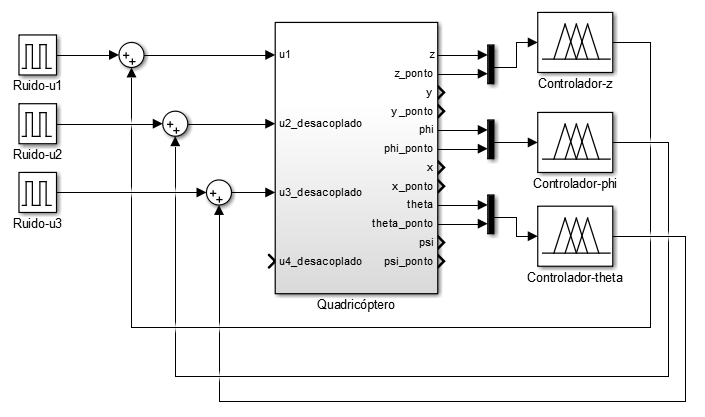
\includegraphics[width=0.8\textwidth]{./04-figuras/figuras_pos_banca/2-sistema_completo_controlado/diagrama_sistema_controlado}
    \label{fig:diagrama_sistema_controlado}
\end{figure}

Como se pode ver, três controladores agem no sistema com o objetivo de torná-lo imune a distúrbios representados pelas entradas de ruídos. O {\ttfamily Controlador-z} diz respeito a um controlador de altitude ao passo que os {\ttfamily Controlador-phi} e {\ttfamily Controlador-theta} dizem respeito a controladores de atitude que, pelo fato de o quadricóptero ser simétrico em relação aos eixos x e y, puderam ser representados por um único controlador.

O controlador de altitude possui duas entradas e uma saída. As entradas são referentes à posição vertical do quadricóptero ($z$) e sua respectiva velocidade ($\dot{z}$), ao passo que a saída diz respeito ao sinal de controle a ser aplicado sobre o sistema para estabilizar sua altitude ($u_1$).

Utilizando o \textit{Fuzzy Logic Toolbox} do MATLAB, cada variável linguística do controlador \textit{fuzzy} foi divida em três conjuntos: N (negativo), Z (zero) e P (positivo), tomando como base os trabalhos de \citeonline{Maj2013} e \citeonline{Gao2014Stability}. As regras \textit{fuzzy} definidas para este controlador são mostradas no Quadro \ref{qua:regras_fuzzy_u1_mamdani}, e a Figura \ref{fig:1_mamdani_surface} exibe seu equivalente em superfície.

% Mostrar regras Fuzzy envolvidas no controle de u1 (quadro de regras + superfície)
\begin{quadro}[!htb]
    \centering
    \caption{Regras fuzzy para modelagem do controle de altitude\label{qua:regras_fuzzy_u1_mamdani}}
    \begin{tabular}{|c|c|c|}
    % \begin{tabular}{>{\centering\bfseries}m{1in} >{\centering}m{1in}
        \hline
        \textbf{{$z$}} & 
        \textbf{{$\dot{z}$}} &
        \textbf{{$u_1$}} \\
        \hline %01
            N &
            - &
            N \\
        \hline %02
            P &
            - &
            P \\
        \hline %03
            Z &
            N &
            N \\
        \hline %04
            Z &
            Z &
            Z \\
        \hline %05
            Z &
            P &
            P \\
        \hline
    \end{tabular}
    % \begin{TAB}(r,1cm,2cm)[5pt]{|c|c|}{|c|c|c|}% (rows,min,max)[tabcolsep]{columns}{rows}
    %     hi & tall one    \\
    %     hi & medium one  \\
    %     hi & standard one\\
    % \end{TAB}
\end{quadro}


\begin{figure}[!htb]
    \centering
    \caption{Superfície das regras do sistema de controle fuzzy para a altitude do quadrotor}
    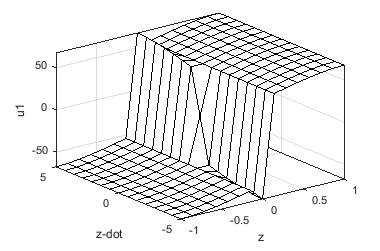
\includegraphics[width=0.6\textwidth]{./04-figuras/resultados/fis_u1/u1_mamdani_surface}
    \label{fig:1_mamdani_surface}
\end{figure}

O controlador de atitude projetado também possui duas entradas e uma saída. Desta vez, entretanto, as entradas são referentes ao ângulo em relação ao eixo horizontal ($\phi$ ou $\theta$) e sua respectiva variação ($\dot{\phi}$ ou $\dot{\theta}$). Mais uma vez, cada variável linguística foi dividida em três conjuntos: N, Z e P.

As regras que regem o controlador de atitude são sintetizadas no Quadro \ref{qua:regras_fuzzy_u2_u3_mamdani} e podem ser vistas na superfície de regras mostradas na Figura \ref{fig:u2_u3_mamdani_surface}.

% Mostrar regras Fuzzy envolvidas no controle de u2 e u3 (quadro de regras + superfície)
\begin{quadro}[!htb]
    \centering
    \caption{Regras fuzzy para modelagem do controle de atitude\label{qua:regras_fuzzy_u2_u3_mamdani}}
    \begin{tabular}{|c|c|c|}
    % \begin{tabular}{>{\centering\bfseries}m{1in} >{\centering}m{1in}
        \hline
        \textbf{{$\phi/\theta$}} & 
        \textbf{{$\dot{\phi}/\dot{\theta}$}} &
        \textbf{{$u_2/u_3$}} \\
        \hline %01
            P &
            P &
            N \\
        \hline %02
            P &
            Z &
            N \\
        \hline %03
            P &
            N &
            Z \\
        \hline %04
            N &
            N &
            P \\
        \hline %05
            N &
            Z &
            P \\
        \hline %06
            N &
            P &
            Z \\
        \hline %07
            Z &
            Z &
            Z \\
        \hline %08
            Z &
            N &
            P \\
        \hline %09
            Z &
            P &
            N \\
        \hline
    \end{tabular}
    % \begin{TAB}(r,1cm,2cm)[5pt]{|c|c|}{|c|c|c|}% (rows,min,max)[tabcolsep]{columns}{rows}
    %     hi & tall one    \\
    %     hi & medium one  \\
    %     hi & standard one\\
    % \end{TAB}
\end{quadro}


\begin{figure}[!htb]
    \centering
    \caption{Superfície das regras do sistema de controle fuzzy para a atitude do quadrotor}
    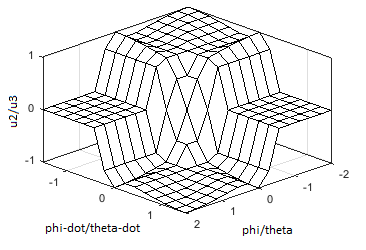
\includegraphics[width=0.6\textwidth]{./04-figuras/resultados/fis_u2/u2_u3_mamdani_surface}
    \label{fig:u2_u3_mamdani_surface}
\end{figure}
